\chapter{Simulation Results}
\label{sec:simulation_results}

The most interesting designs described in \Cref{sec:optimization_results} are
tested in simulation. As explained in \Cref{sec:method}, they are simulated in
Gazebo$^\textrm{\textregistered}$ and controlled by the means of a ROS node.
This chapter first presents a flight test performed by the tri-copter depicted in
\Cref{fig:comp_tri}, then a comparison between the hexa-copter shown in
\Cref{fig:comp_hexa} and the Voliro from \citep{kamel_voliro:_2018}
is proposed. Finally, a manipulation example with the hepta-copter
presented in \Cref{sec:hepta_copter} is shown.

\section{Tri-copter}
\label{sec:tri_copter_sim}

The tri-copter with tilting rotor is a very interesting case because it is holonomic,
which means that it has exactly six degrees of freedom (DoF) and evolves in a
three dimensional space. Therefore, it should theoretically be able to produce forces
and torques in any direction. To verify that a test flight is performed where the MAV
hover at one meter over the ground and changes its orientation up to a pitch angle
$\theta$ equal to $90^{\circ}$. The results of this test can be observed in
\Cref{fig:tri_sim} and it is clear from this quarter pitch flip that the tri-copter
is indeed able to hover in any orientation.\\

\begin{figure}[!ht]
  \begin{center}
  \begin{minipage}[t]{0.24\textwidth}
    \centering
    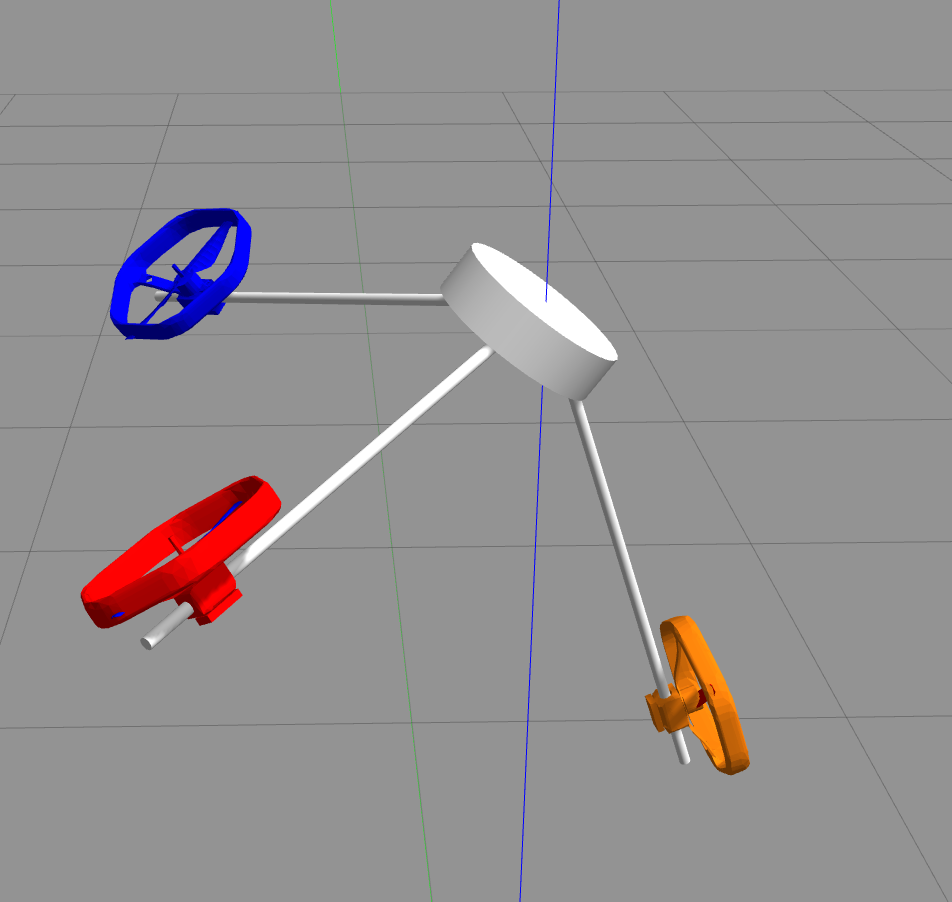
\includegraphics[width=\linewidth]{images/tri_sim1.png}
  \end{minipage}
  \hfill
  \begin{minipage}[t]{0.24\textwidth}
    \centering
    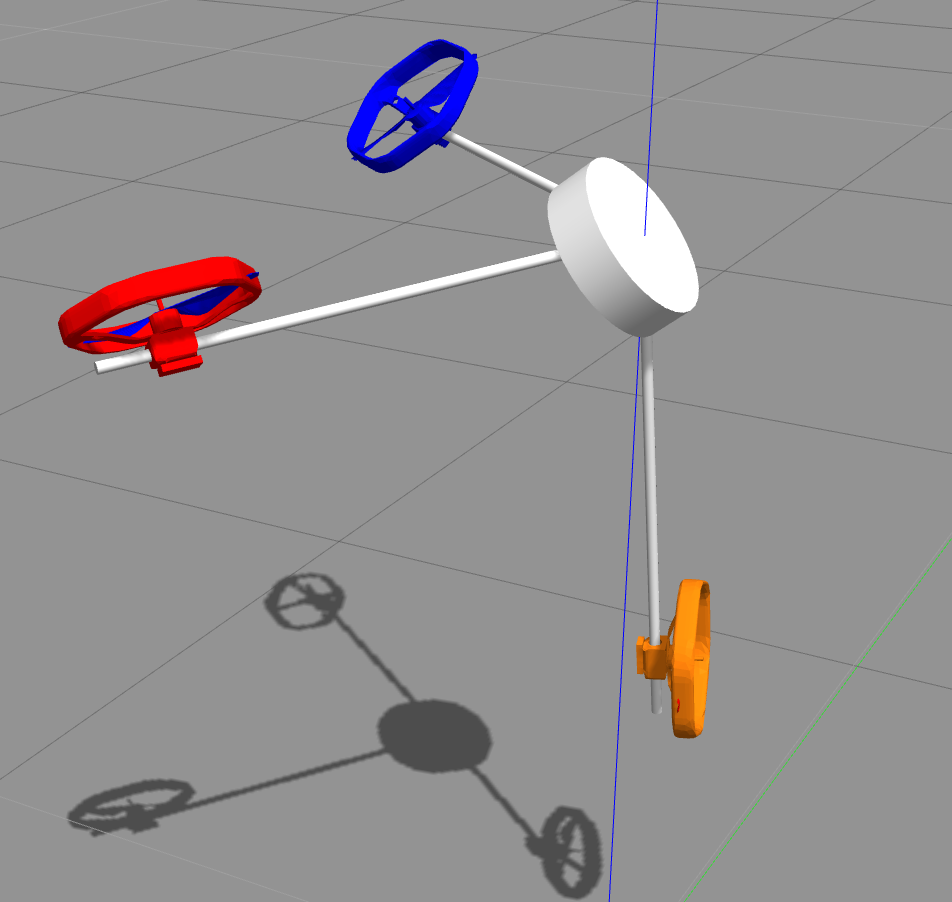
\includegraphics[width=\linewidth]{images/tri_sim2.png}
  \end{minipage}
  \hfill
  \begin{minipage}[t]{0.24\textwidth}
    \centering
    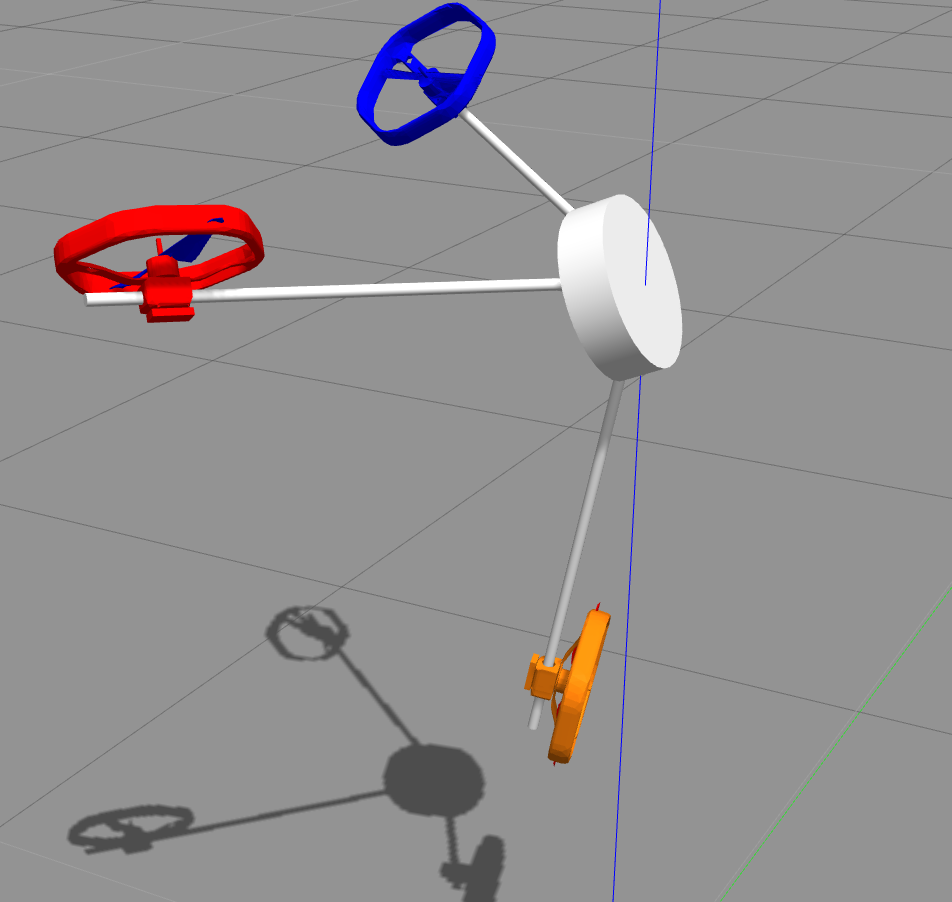
\includegraphics[width=\linewidth]{images/tri_sim3.png}
  \end{minipage}
  \hfill
  \begin{minipage}[t]{0.24\textwidth}
    \centering
    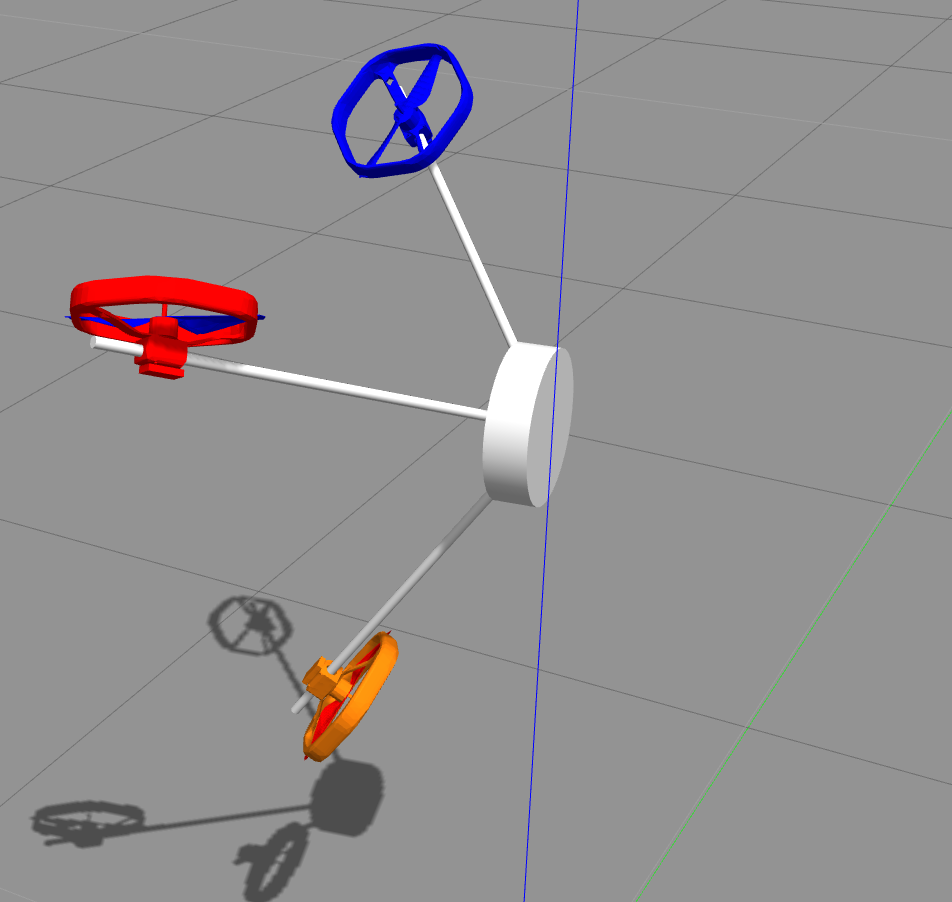
\includegraphics[width=\linewidth]{images/tri_sim4.png}
  \end{minipage}
  \caption{Simulation of the tri-copter in Gazebo.}
  \label{fig:tri_sim}
  \end{center}
\end{figure}

\clearpage

\section{Hexa-copter}
\label{sec:hexa_copter_sim}

\begin{figure}[!ht]
  \resizebox{\textwidth}{!}{\begin{subfigure}[b]{0.5\textwidth}
    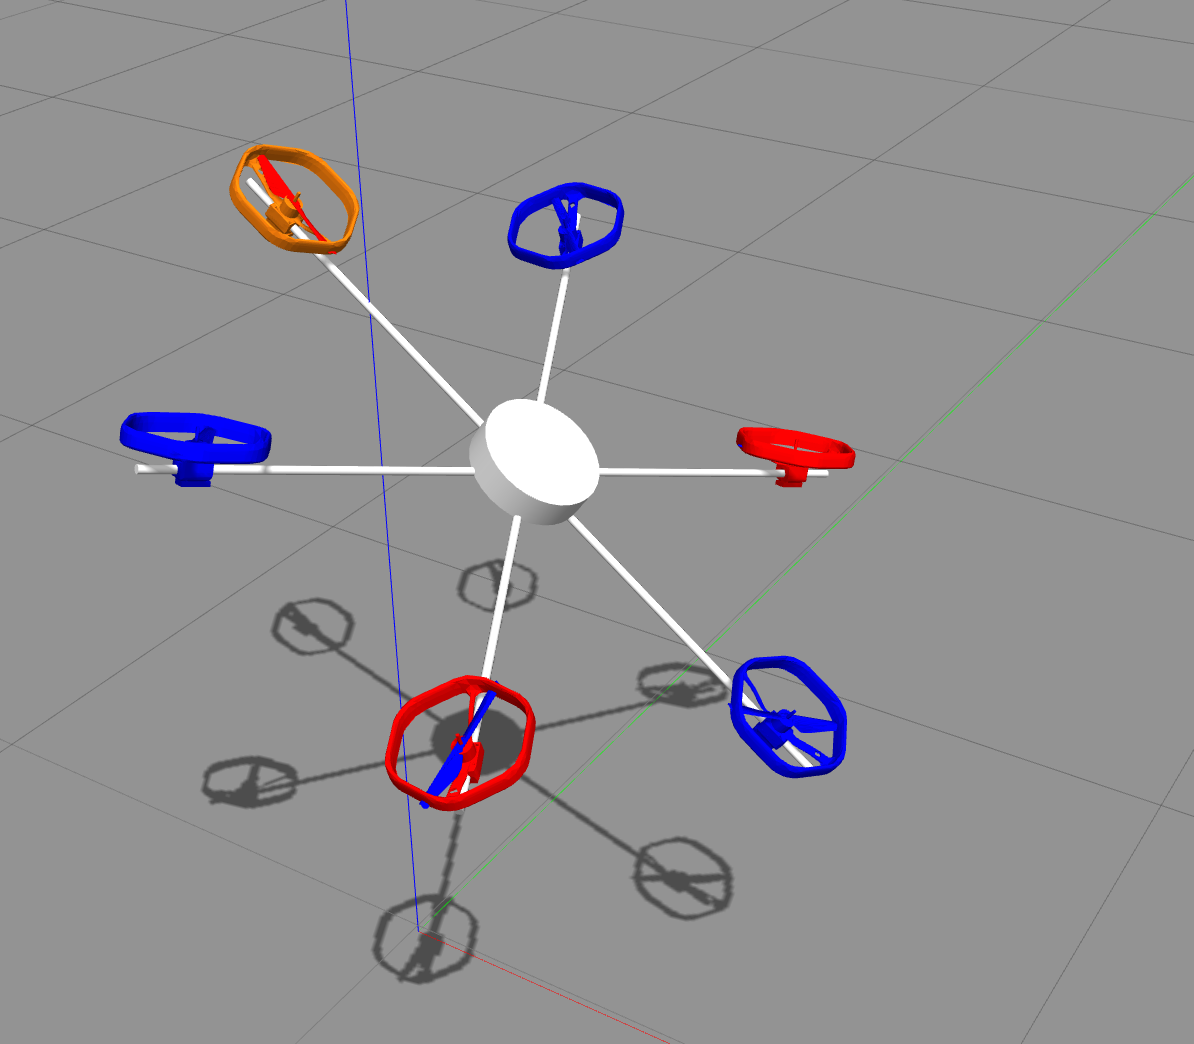
\includegraphics[width=\linewidth]{images/Voliro_sim.png}
    \caption{Voliro.} \label{fig:Voliro_sim}
  \end{subfigure}
  \hspace*{\fill} % separation between the subfigures
  \begin{subfigure}[b]{0.5\textwidth}
    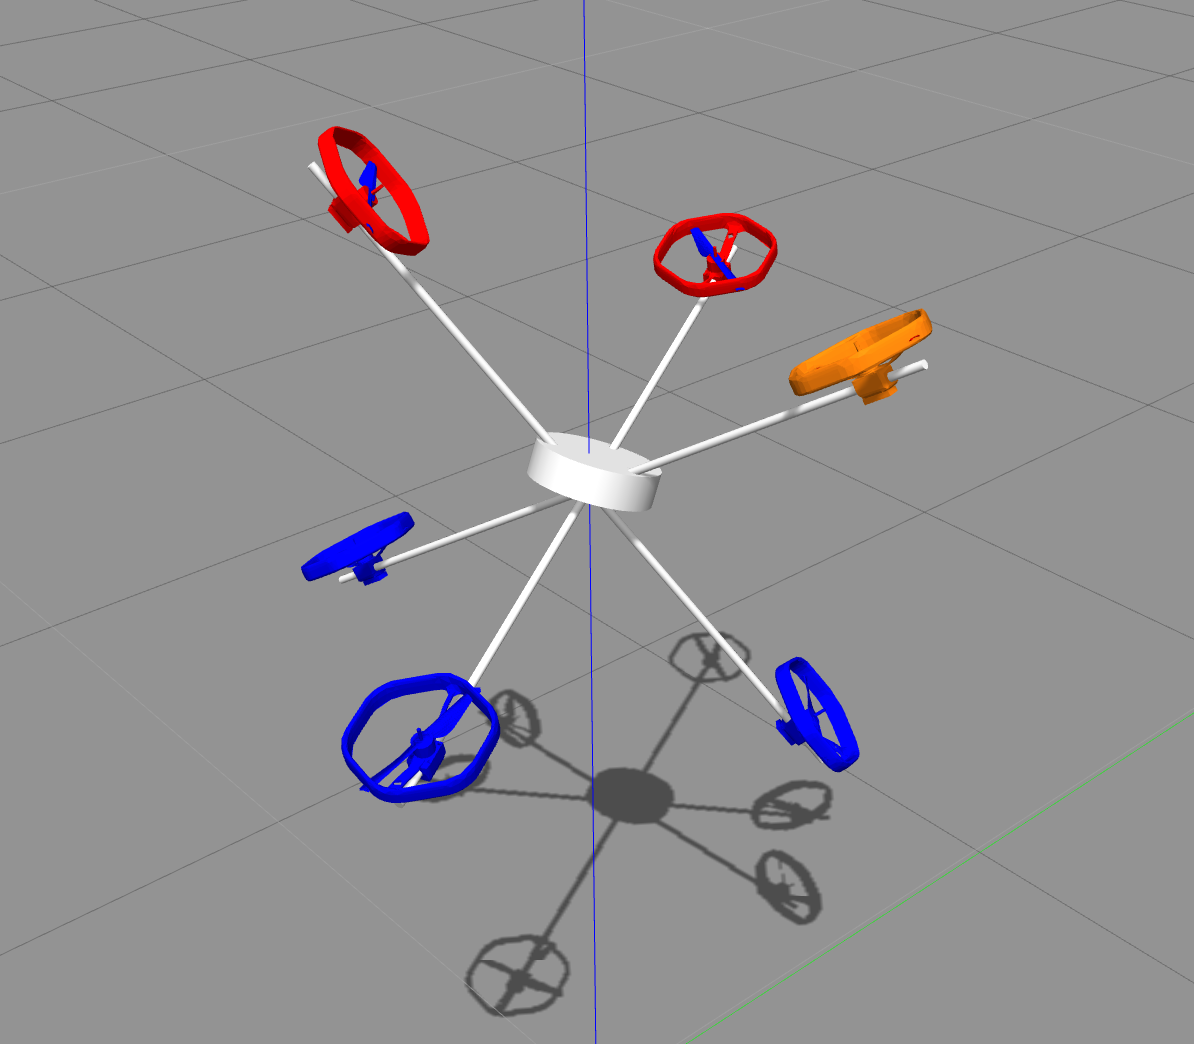
\includegraphics[width=\linewidth]{images/Hexa_sim.png}
    \caption{Optimal hexa-copter.} \label{fig:Hexa_sim}
  \end{subfigure}}
  \caption{Angle error.}
  \label{fig:Sim_six_rotors}
\end{figure}

\begin{figure}[!ht]
  \centering
  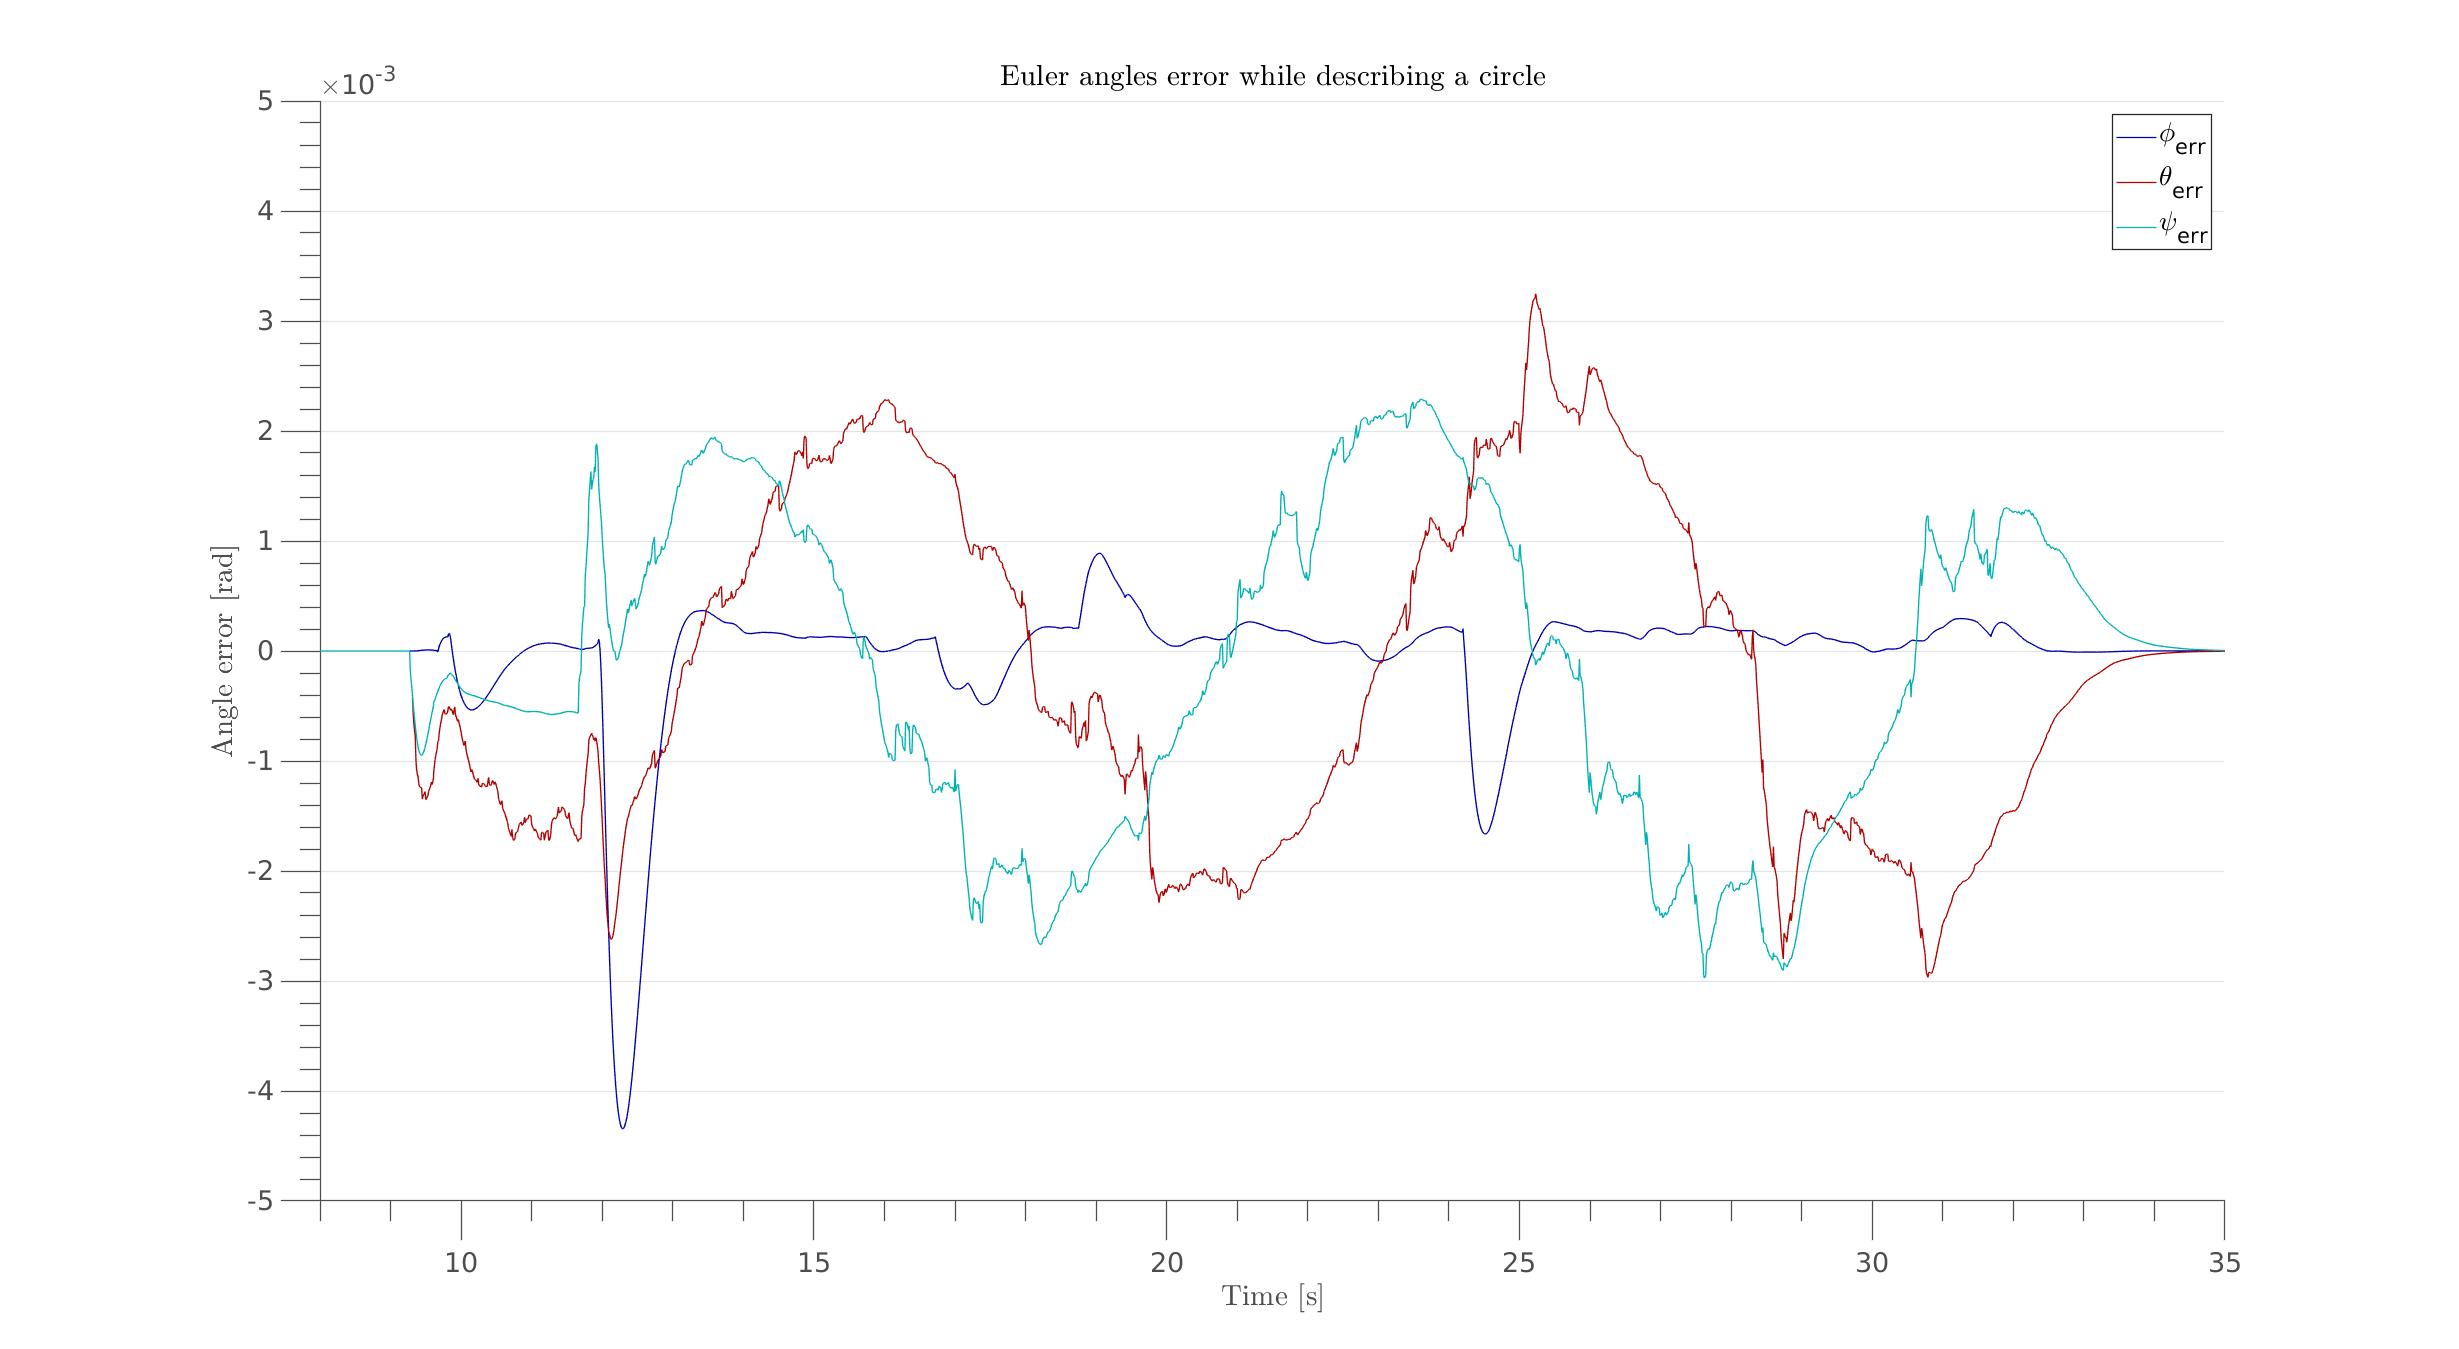
\includegraphics[width=\linewidth]{images/Voliro_circle_angle.jpg}
  \caption{Angle error.}
  \label{fig:Voliro_angle_error_circle}
\end{figure}

However, the controller uses
the static allocation described in \Cref{sec:allocation} to compute the desired
tilting angles and speed for the rotors. This leads to the loss of full-actuation in
certain orientations where the static allocation matrix becomes singular.

\section{Hepta-copter}
\label{sec:hepta_copter_sim}
